\documentclass{template/openetcs_report}
% Use the option "nocc" if the document is not licensed under Creative Commons
%\documentclass[nocc]{template/openetcs_article}
\usepackage{lipsum,url}
\usepackage{supertabular}
\usepackage{multirow}
\usepackage{color, colortbl}
\definecolor{gray}{rgb}{0.8,0.8,0.8}
\usepackage[modulo]{lineno}
\graphicspath{{./template/}{.}{./images/}}

\begin{document}
\frontmatter
\project{openETCS}

%Please do not change anything above this line
%============================
% The document metadata is defined below

%assign a report number here
\reportnum{OETCS/WP4/D4.3.3V0.0}

%define your workpackage here
\wp{Work-Package 4: ``Validation \& Verification Strategy''}

%set a title here
\title{openETCS Safety case for tool chain and processes}

%set a subtitle here
\subtitle{Process and Toolchain verification for the openETCS on-board unit software development}

%set the date of the report here
\date{November 2015} %\\ Revised April 2015}

%document approval
%define the name and affiliation of the people involved in the documents approbation here
\creatorname{Jan Welte]}
\creatoraffil{TU Braunschweig}

\techassessorname{Abdelnasir Mohamed}
\techassessoraffil{AEbt}

\qualityassessorname{Veronique Gontier}
\qualityassessoraffil{All4Tec}

\approvalname{Klaus-R\"udiger Hase}
\approvalaffil{DB Netz}

%define a list of authors and their affiliation here

\author{Jan Welte}

\affiliation{Technische Universität Braunschweig\\
  Institute for Traffic Safety and Automation Engineering\\
  Hermann-Blenk-Str. 42\\
  38108 Braunschweig, Germany\\
  eMail: openetcs@iva.ing.tu-bs.de \\
  WebSite: www.iva.ing.tu-bs.de}
  
  
%add yourself as author, if you contributed to the document



% define the coverart
\coverart[width=350pt]{openETCS_EUPL}

%define the type of report
\reporttype{Output Document}


\begin{abstract}
This document addresses the general quality and safety assurance concept implemented and used by the openETCS development process and its respective toolchain. 

\end{abstract}

%=============================
%Do not change the next three lines
\maketitle
\tableofcontents
\listoffiguresandtables
\newpage
%=============================

\chapter{Document Control}

\begin{tabular}{|p{4.4cm}|p{8.7cm}|}
\hline
\multicolumn{2}{|c|}{Document information} \\
\hline
Work Package &  WP4  \\
Deliverable ID & D 4.3.3\\
\hline
Document title & Process and Toolchain verification for the openETCS on-board unit software development \\
Document version & 0.1 \\
Document authors (org.)  & Jan Welte (TU-BS)\\
\hline
\end{tabular}

\begin{tabular}{|p{4.4cm}|p{8.7cm}|}
\hline
\multicolumn{2}{|c|}{Review information} \\
\hline
Last version reviewed & \\
\hline
Main reviewers (org.) & \\
\hline
\end{tabular}

\begin{tabular}{|p{2.2cm}|p{4cm}|p{4cm}|p{2cm}|}
\hline
\multicolumn{4}{|c|}{Approbation} \\
\hline
  &  Name & Role & Date   \\
\hline  
Written by    &  Jan Welte & WP4-T4.4 Task Leader  &  November 2015\\
\hline
Approved by & -- & -- & \\
\hline
\end{tabular}

\begin{tabular}{|p{2.2cm}|p{2cm}|p{3cm}|p{5cm}|}
\hline
\multicolumn{4}{|c|}{Document evolution} \\
\hline
Version &  Date & Author(s) & Justification  \\
\hline
0.1 & 18/10/2013 & Jan Welte &  Document creation \\
\hline  
%0.1 & 28/01/2014 & Jan Welte &  Extended Introduction  \\
\hline  
\end{tabular}
\newpage

% The actual document starts below this line
%=============================

\mainmatter

\chapter{Introduction}
\label{sec:introduction}

..

\section{Purpose}
\label{sec:purpose}

...

\section{Document Structure}
\label{sec:document-structure}

...

\section{Document Evolution}

...

\section{Reference Documents}
\label{sec:refdoc}

This document essentially refers to the following standards, ETCS specification documents and openETCS project documents.

\begin{itemize}
\item \textbf{ISO~9000} --- 12/2005 --- \emph{Quality management}
\item \textbf{ISO~9001} --- 12/2008 --- \emph{Quality management systems — Requirements}
\item \textbf{ISO~25010} --- 03/2011 --- \emph{Systems and software engineering -- Systems and software Quality Requirements and Evaluation (SQuaRE) -- System and software quality models}
\item \textbf{CENELEC EN~50126-1} --- 01/2000 --- \emph{Railways applications –- The specification and 
demonstration of Reliability, Availability, Maintenability and Safety (RAMS) –- Part 1: 
Basic requirements and generic process}
\item \textbf{CENELEC EN~50128} --- 10/2011 --- \emph{Railway applications -- Communication, signalling and 
processing systems -- Software for railway control and protection systems}
\item \textbf{CENELEC EN~50129} --- 05/2003 --- \emph{Railway applications –- Communication, signalling and 
processing systems –- Safety related electronic systems for signalling}
\item \textbf{CCS~TSI} --- \emph{ CCS TSI for HS and CR transeuropean rail has been adopted by a Commission Decision 2012/88/EU on the 25th January 2012}
\item \textbf{SUBSET-026} 3.3.0 --- \emph{System Requirement Specification}
\item \textbf{SUBSET-091} 3.2.0 --- \emph{Safety Requirements for the Technical Interoperability
of ETCS in Levels 1 \& 2}
\item \textbf{SUBSET-088} 2.3.0 --- \emph{ETCS Application Levels 1 \& 2 - Safety Analysis}
\item \textbf{OpenETCS FPP} --- \emph{Project Outline Full Project Proposal Annex OpenETCS} -- v2.2
\item \textbf{OpenETCS D2.2} -- Report on CENELEC standard
\item \textbf{OpenETCS D2.3} -- Definition of the overall process for the formal description of ETCS and the rail system it works in 
\item \textbf{OpenETCS D2.4} -- Definition of the methods used to perform the formal description
\end{itemize}


%%%%%%%%%%%%%%%%%%%%%%%%%%%%%%%%%%%%%%%%%%%%%%%%%%%%%%%%%%%%%%%

\section{Glossary}
\label{sec:glossary}



\begin{tabular}{rl}
\textbf{ACedit} & Assurance Case Editor \\ 
\textbf{ARM} & Argumentation  Metamodel \\ 
\textbf{ETCS} & European Train Control System \\ \textbf{ERA} & European Railway Agency \\ \textbf{FMEA} & Failure Mode Effect Analysis \\ 
\textbf{GSN} & Goal Structured Notation \\ 
\textbf{MoRC} & Management of Radio Communication \\ 
\textbf{RAMS} & Reliability, Availability, Maintainability and Safety \\
\textbf{SIL} & Safety Integrity Level \\ 
\textbf{SRS} & System Requirement Specification \\ 
\textbf{THR} & Tolerable Hazard Rate \\ 
\textbf{V\&V} & Verification \& Validation \\ 
\end{tabular} 




\section{Background Information}
\label{sec:Background}


If specific information are needed the can be place here. (D4.2.3 shall not be repeated)


\chapter{Tool Chain}

\section{overview}

by Jan Welte

\section{Tool Qualification}

by Michael Jastram (or other expert from WP7)


broad overview of the toolchain and the status of qualification (generall information can be placed in section Overview)
- which tools have to be qualified
- which tools are qualified? (in which way)
- how should qualification be address for tools with pending qualification

\section{SCADE}

by Jan Welte and Marc Behrens

- use of SCADE for quality assurance
- limitations of SCADE
- addressing safety issues and properties in SCADE 
(potential specific aspects in openETCS deviation from the usual use of SCADE)


\section{Safety Architect}

by FrederiqueVallee (or Francois Revest)

- use of Safety Architect in openETCS (maybe addressing relation to Eclipse Safety Framework)
- function in development process
- inputs and outputs
- results (in general, and specific for openETCS)

\chapter{OpenETCS Development}
\label{sec:development-process}

\section{overview}

by Jan Welte

Short overview of current work.

- Main principals to ensure consistency 

- Mainly collecting findings

- allocate the tools to the process steps used/ qualified

\section{Compatibility to CENELEC standards}

by Mohamed Abdelnasir

- overview results relation to EN 50126/50128 lifecycle 
- reasons for deviations
- additional findings

\section{Traceability}

by @janwelte @raphaelfaudou

- addressing specific position of traceability for safety argumentation
- introducing basic concept
- main findings (limitations)

Requirement traceability activity consists in ensuring that all product engineering artifacts (including verification means) can be traced to an originating stakeholder requirement either directly (direct link) or through other requirements derived from stakeholder requirements. It means creating links but also manage their status (created, confirmed...) and potentially their deletion.

Concerning OpenETCS, there are several needs for traceability but main ones concern definition of links between SRS-Subset 26 requirements and two models:
\begin{itemize}
\item OpenETCS architecture SysML model (System, subsystem, SW functions), edited with SCADE System tool
\item OpenETCS OBU formal executable software model (SW architecture, SW functions, detailed design), edited with SCADE Suite tool
\end{itemize}

Figure \ref{fig:openETCSTraceabilityMainPriority} illustrates all required traceability links needed to achieve current design verification and highlights main priority (arrows with largest size).

\begin{figure}[htbp]
\centering
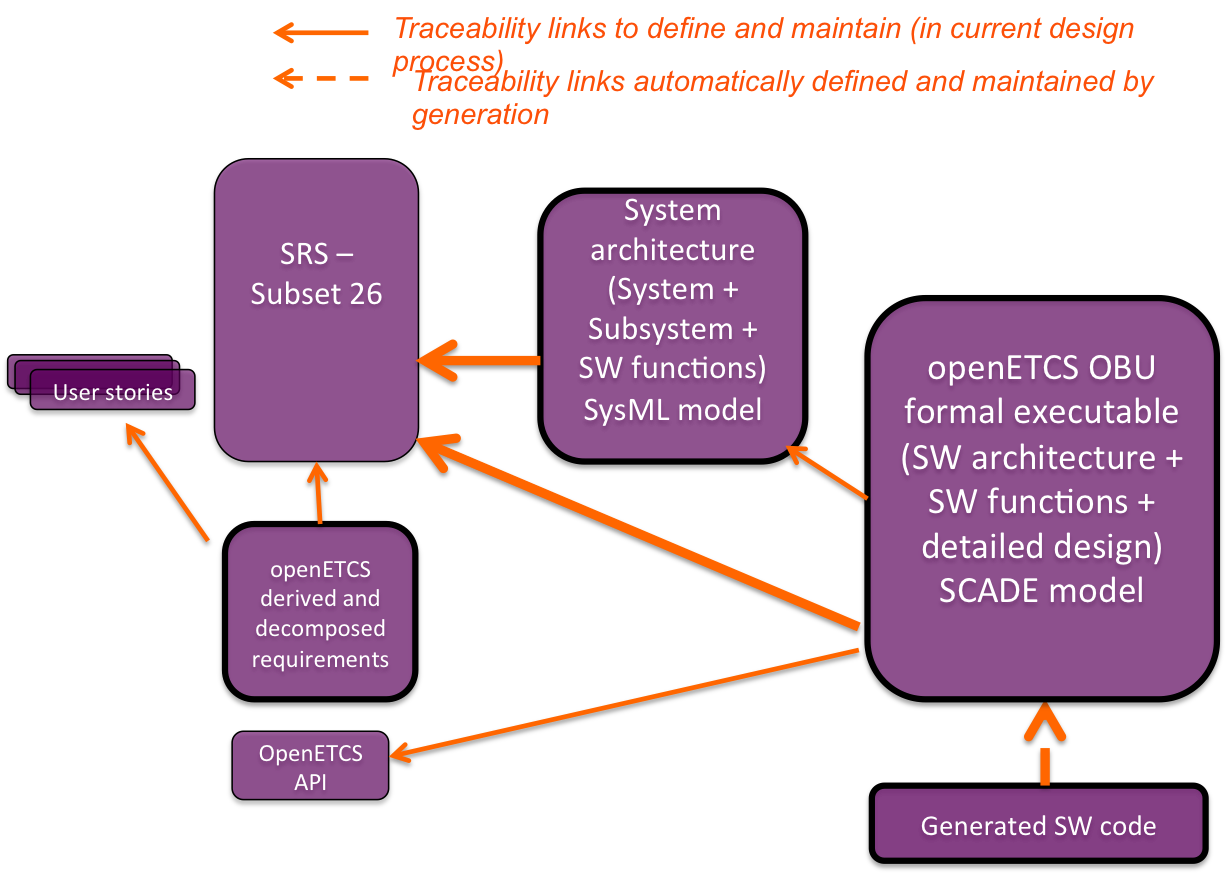
\includegraphics[width=.9\linewidth]
{./images/openETCSTraceabilityMainPriority.png}
\caption{\label{fig:openETCSTraceabilityMainPriority}OpenETCS traceability chains for current design with highlight on main priorities}
\end{figure}

OpenETCS tool chain currently supports ability to create links between:
\begin{itemize}
\item SRS Subset 026 .ReqIF requirements and additional requirements => through ProR integrated tool,
\item SysML architecture model and SRS Subset 026 .ReqIF requirements through ReqCycle integrated tool
\end{itemize}
 
\textbf{Note:} it is also possible to create links between SCADE Model and SRS Subset 026 .ReqIF requirements through SCADE Suite RM Gateway and ReqTify traceability product but it is not an open solution and it requires additional licenses. Therefore that approach was used only by a few partners and was not considered as conclusive. There are pending investigations to provide alternate open solutions to support edition of those traceability links.




\chapter{Generic OpenETCS Safety Case}
\label{sec:hazardandrisk}

\section{System/ Sub-System Definition}

by Jan Welte

- general information concerning openETCs system and sub-system structure
- potential applications for artifacts

\section{Quality Management}

by Mohamed Abdelnasir

- basic concept for quality management in openETCS
- missing aspects in quality management
- main finding to address additional measures to complete quality management

\section{Safety Management}

by Jan Welte

- basic concept for safety management in openETCS
- missing aspects in safety management
- main finding to address additional measures to complete safety management

\section{Functional/Technical Safety}
by Jan Welte

- addressing general system safety properties and allocation to functional structure
- listing needed integration properties for "safe" use of software model (specifically interface assumptions)

by Francois Revest

- addressing concrete findings from safety propagation analysis
- additional measures applicable to tackle open points


\chapter{Conclusion}
\label{sec:conclusion}

This document presents the final results ...

\bibliographystyle{unsrt}
\bibliography{./ref/ref-HaRA}


%===================================================
%Do NOT change anything below this line

\end{document}


